Use pandas to get general summary of protein lengths.

~\begin{figure}[h!]
	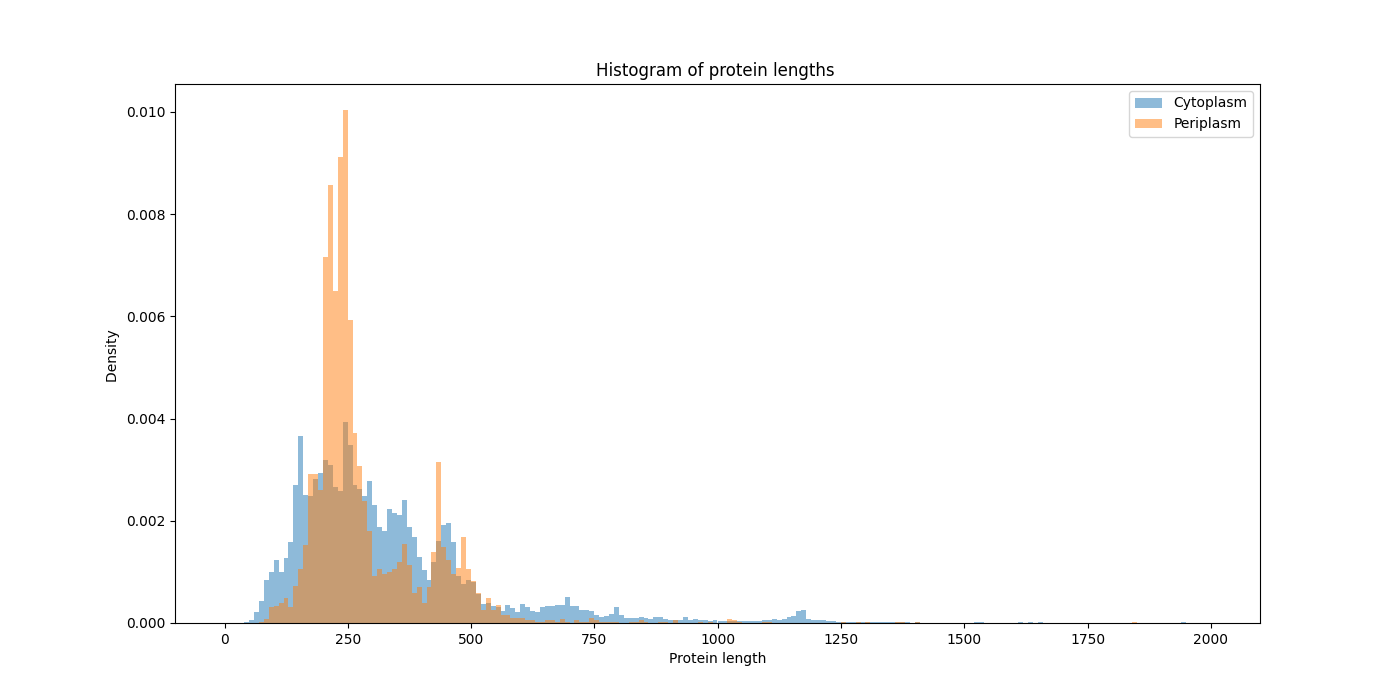
\includegraphics[width=\linewidth]
	{./results/general_comparison/img/protein_length.png}
~\end{figure}

~\begin{figure}[h!]
	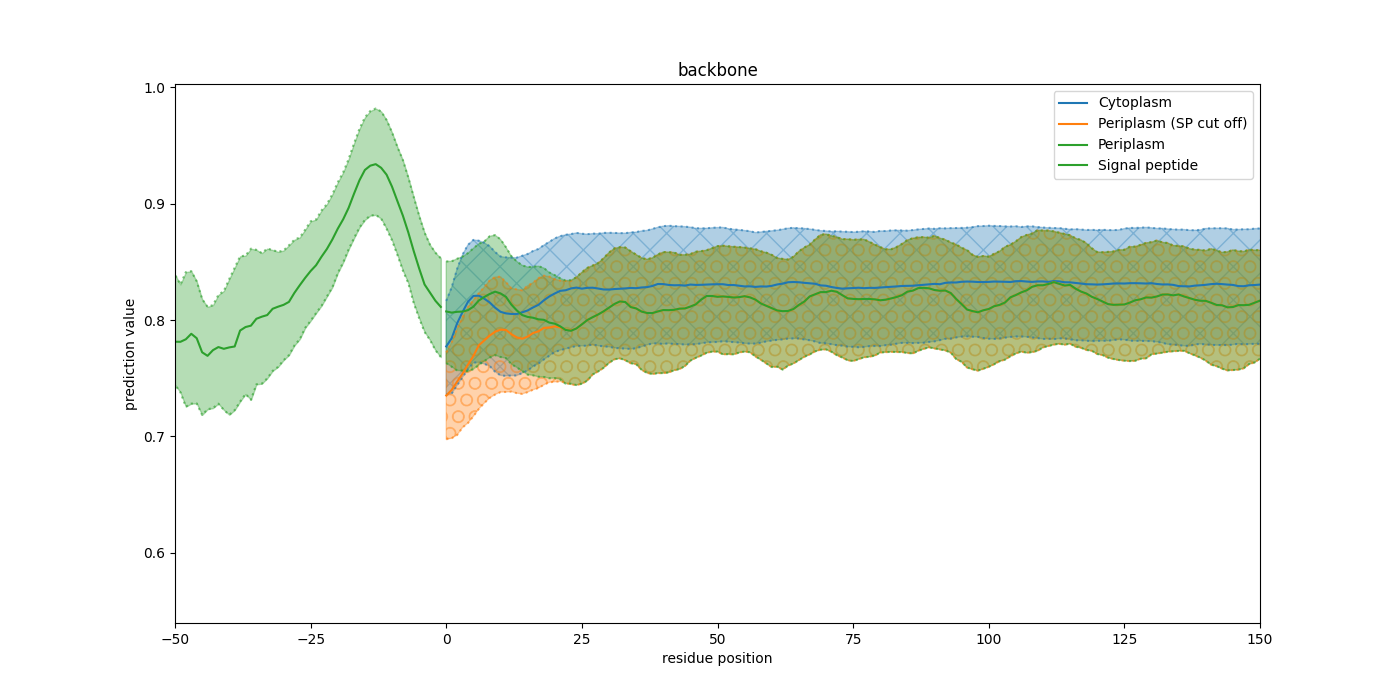
\includegraphics[width=\linewidth]
	{./results/general_comparison/img/backbone.png}
~\end{figure}

~\begin{figure}[h!]
	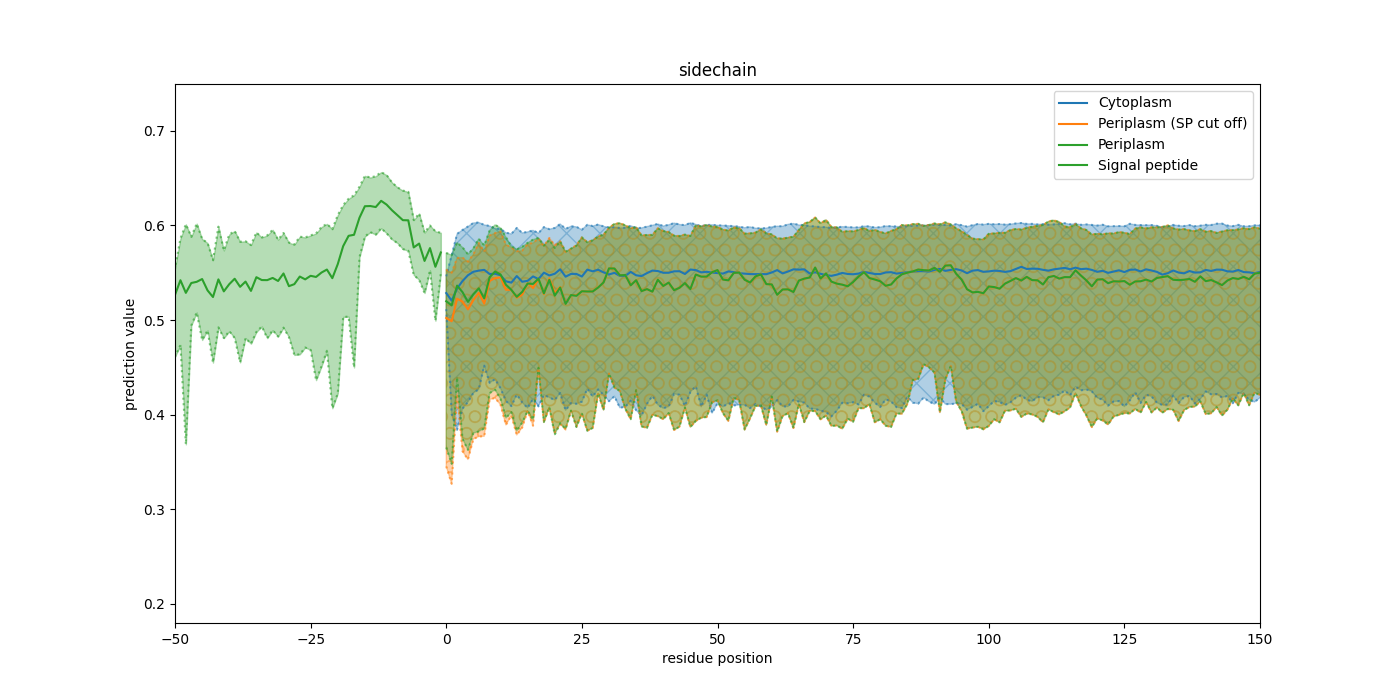
\includegraphics[width=\linewidth]
	{./results/general_comparison/img/sidechain.png}
~\end{figure}

~\begin{figure}[h!]
	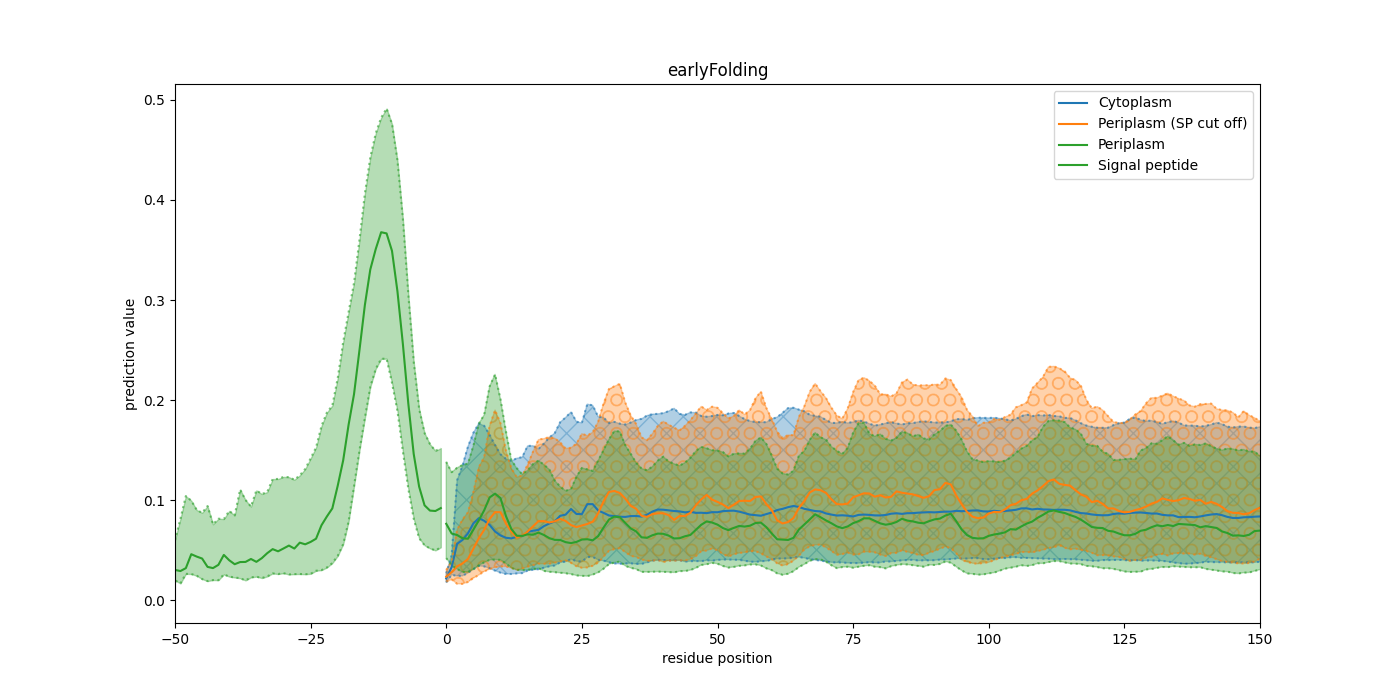
\includegraphics[width=\linewidth]
	{./results/general_comparison/img/earlyFolding.png}
~\end{figure}

~\begin{figure}[h!]
	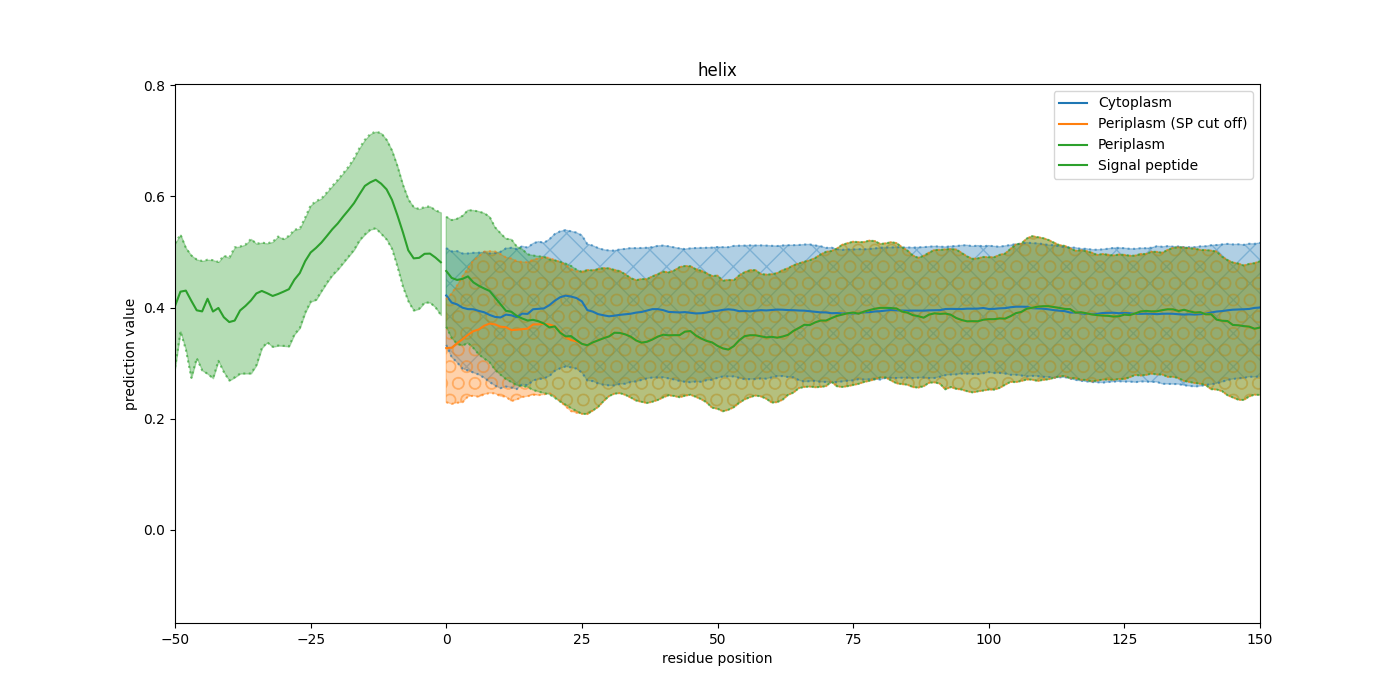
\includegraphics[width=\linewidth]
	{./results/general_comparison/img/helix.png}
~\end{figure}

~\begin{figure}[h!]
	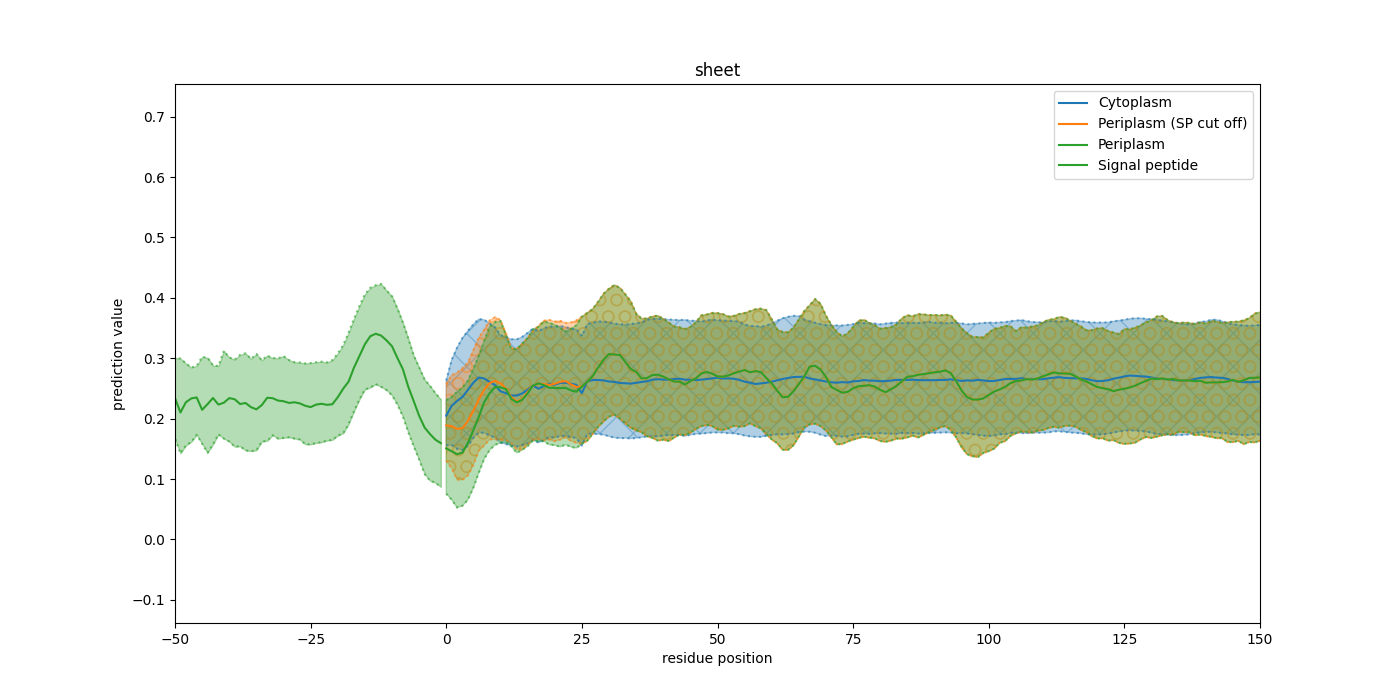
\includegraphics[width=\linewidth]
	{./results/general_comparison/img/sheet.png}
~\end{figure}

~\begin{figure}[h!]
	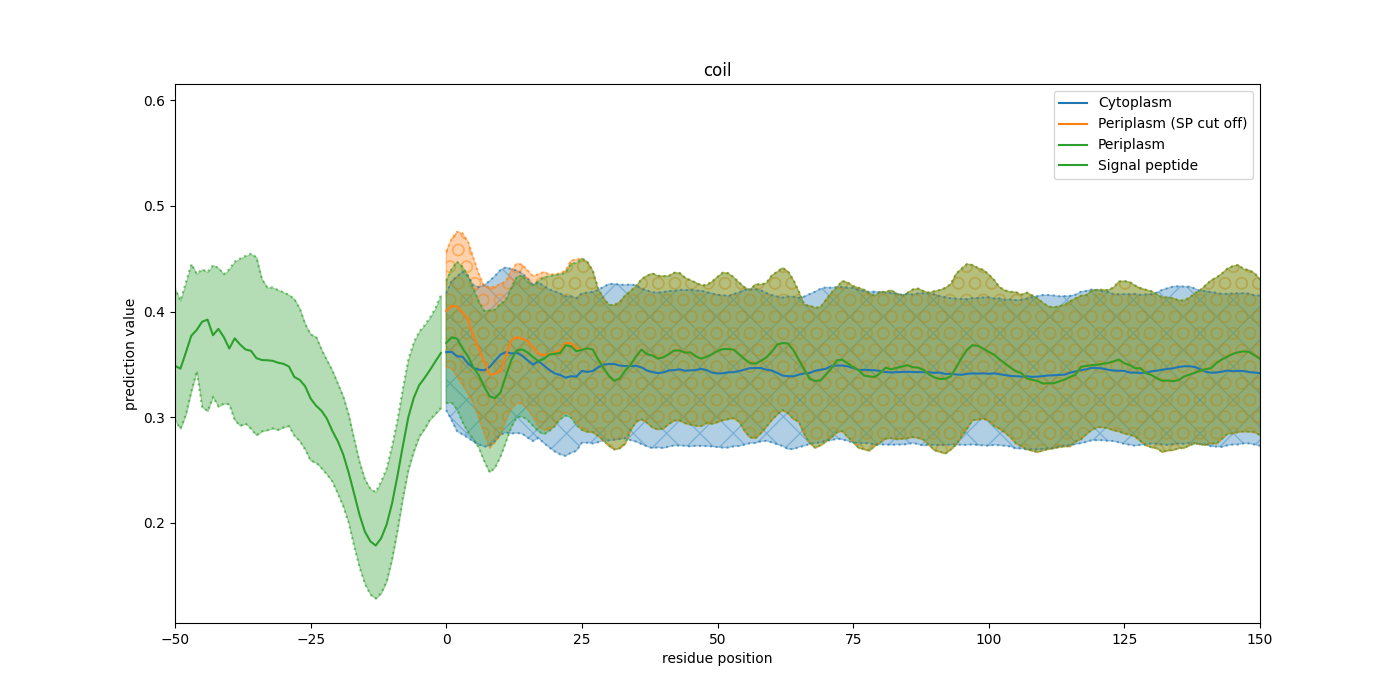
\includegraphics[width=\linewidth]
	{./results/general_comparison/img/coil.png}
~\end{figure}

~\begin{figure}[h!]
	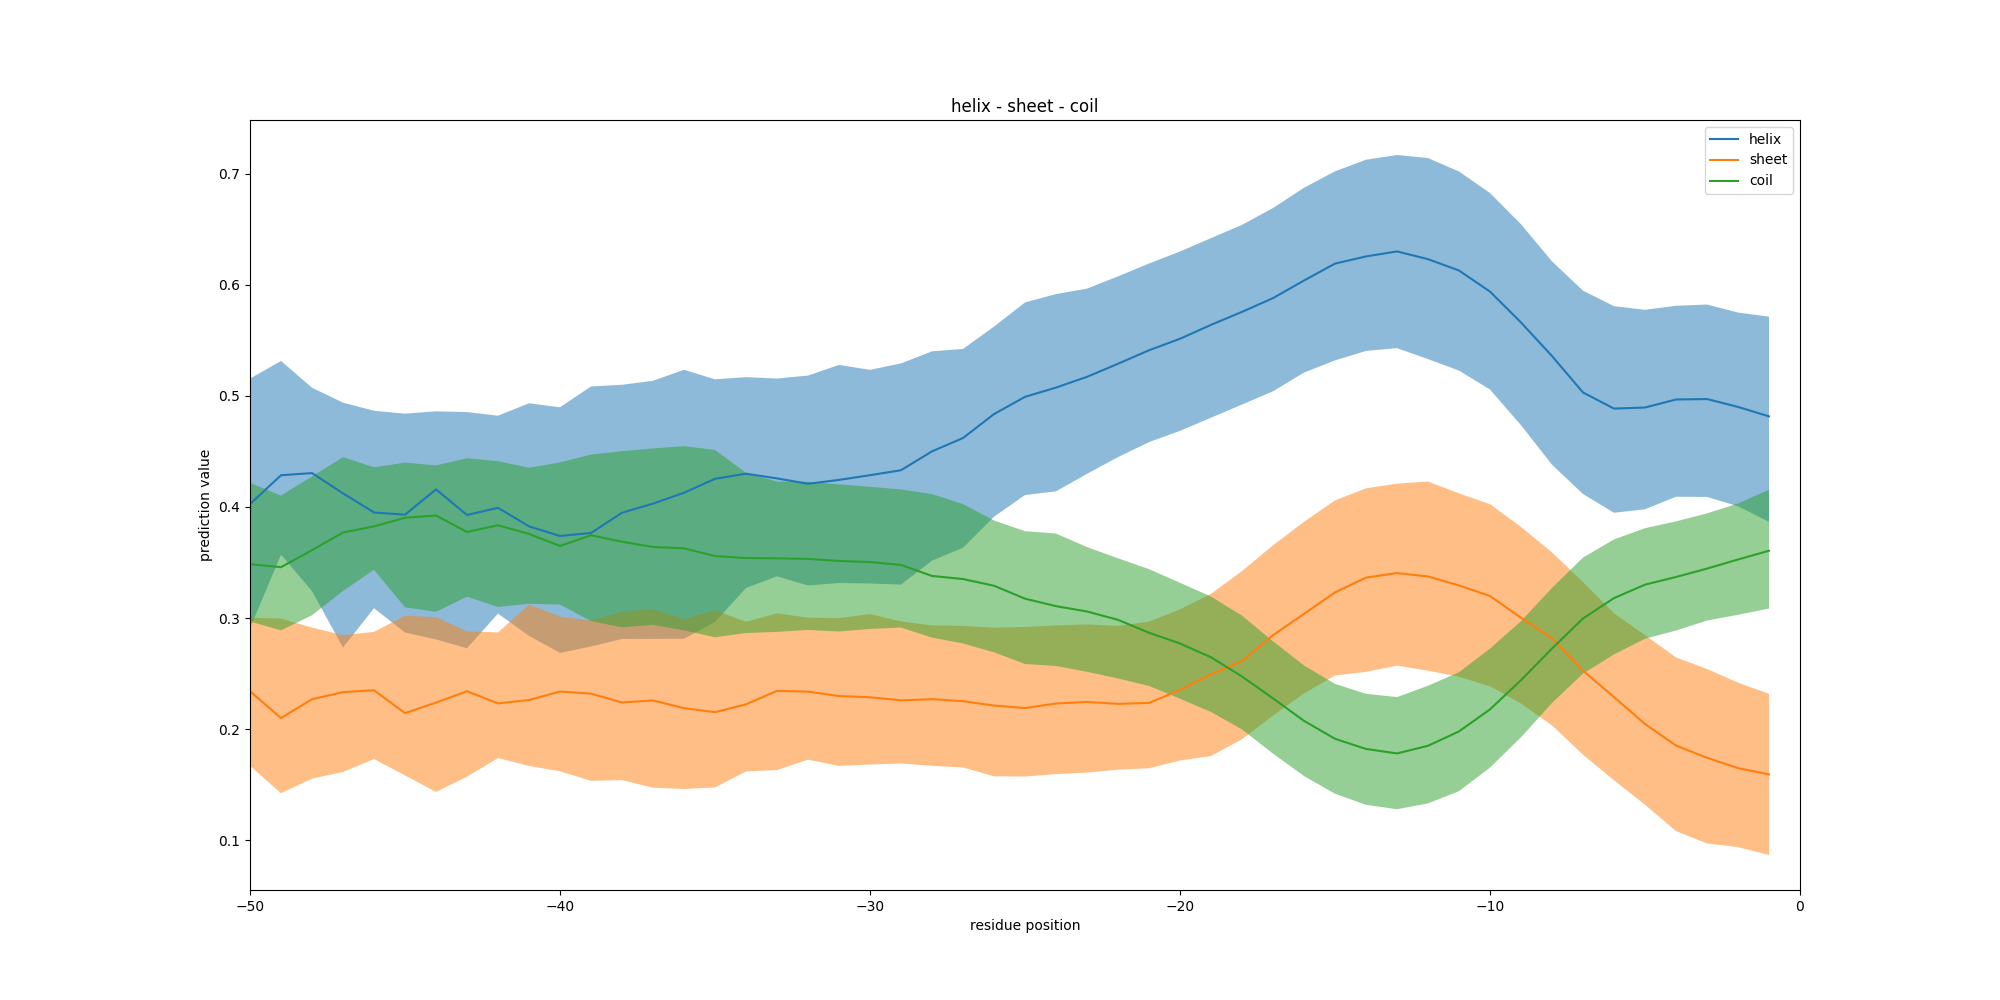
\includegraphics[width=\linewidth]
	{./results/general_comparison/img/signal_peptide.png}
~\end{figure}
